\documentclass{utsignal}

\usepackage{amsmath}
\usepackage{amssymb}
\usepackage{wrapfig}
\usepackage{verbatim}
\usepackage{fancyvrb}
\usepackage{lscape}
\usepackage{rotating}
\usepackage{xepersian}
\usepackage{listings}
\usepackage{color}
\usepackage[utf8]{inputenc}
\usepackage{csquotes}

\title{پروژه - فاز ۱}
\course{سیگنال‌ها و سیستم‌ها}
\author{\href{mailto:h.barkhordarpour@ut.ac.ir?subject=[SS\%20S98 A2]}{هدی برخوردارپور}، 
\href{mailto:ranjbar.ali@ut.ac.ir?subject=[SS\%20S98 A2]\%20}{علی رنجبر}}
%\lecturer{امیرمسعود ربیعی}
\deadline{جمعه ۲۳ فروردین ۱۳۹۸، ساعت ۲۳:۵۵}
\graphicspath{{./images/}}


\begin{document}
	\maketitle
	\section*{کلیات پروژه}
	در این پروژه می‌خواهیم برنامه‌ای مانند شازم \LTRfootnote{Shazam}برای جستجوی قطعه‌هایی از آهنگ در بین پایگاه داده‌ای از آهنگ‌ها بنویسیم. روش اصلی به صورت زیر است:
	\begin{enumerate}
		\item ساخت یک پایگاه داده از ویژگی‌های هر آهنگ با طول کامل
		\item استخراج ویژگی‌های متناظر برای قطعه‌ی آهنگ (کلیپ صوتی) که باید در بین آهنگ‌های پایگاه داده شناسایی شود.
		\item جستجوی پایگاه داده برای یافتن مطابقت بین ویژگی‌‌های قطعه آهنگ با ویژگی‌های ذخیره شده در پایگاه داده
	\end{enumerate}
	مانند شازم، ویژگی‌های هر آهنگ (یا کلیپ صوتی) جفت پیک‌های مجاور در اسپکتروگرام آهنگ (یا کلیپ صوتی) خواهد بود. پس با پیدا کردن پیک‌های اسپکتروگرام شروع می‌کنیم و با رسم محل این پیک‌ها به دیاگرام تصمیم گیری \LTRfootnote{Constellation map} می‌رسیم. هر پیک در یک زمان و فرکانس مشخص	 \lr{(t, f)} اتفاق می‌افتد و یک دامنه \lr{(A)} دارد. سپس جفت پیک‌هایی که در فاصله‌ی زمانی و فرکانسی مشخصی از هم قرار دارند، در پایگاه داده ذخیره می‌کنیم. برای مثال، اگر دو پیک در $(f_1, t_1)$ و $(f_2, t_2)$ داشته باشیم، ممکن است $(f_1, f_2, t_1, t_2-t_1,A_1,A_2,songid)$ را ذخیره کنیم. اما نمی‌خواهیم همه‌ی جفت پیک‌های ممکن را ذخیره کنیم چون تعداد آن‌ها بسیار زیاد است. بعدا نحوه‌ی انتخاب این پیک‌ها را توضیح می‌دهیم.
	
	بجای $(f_1, _f2, t_1, t_2-t_1,A_1,A_2,songid)$، اندازه‌ها را حذف کرده و فقط $(f_1, f_2, t_1, t_2-t_1,songid)$ را ذخیره می‌کنیم. دلیل این کار در \href{https://www.ee.columbia.edu/~dpwe/papers/Wang03-shazam.pdf}{مقاله} بیان شده است. به صورت خلاصه: ممکن است دامنه‌ی پیک نسبت به تغییرات بهره در فرکانس، مقاوم نباشد.
	
	هر آهنگ به صورت یک جدول از ویژگی‌ها خلاصه می‌شود. این خلاصه مانند یک اثر انگشت برای آهنگ است.
	\begin{center}
		\begin{latin}
			\begin{tabular}{|c|c|c|c|c|}
				$f_1$ & $f_2$ & $t_1$ & $t_2-t_1$ & songid\\
				&&&\vdots&\\
				$f_j$ & $f_k$ & $t_j$ & $t_k-t_j$ & songid\\
				&&&\vdots&\\
				$f_m$ & $f_n$ & $t_m$ & $t_n-t_m$ & songid\\
			\end{tabular}
		\end{latin}
	\end{center}
	برای هر کلیپ صوتی نیز همان مراحل استخراج ویژگی‌ها را انجام می‌دهیم و جدولی مانند زیر بدست می‌آوریم:
	\begin{center}
		\begin{latin}
			\begin{tabular}{|c|c|c|c|}
				$f_1$ & $f_2$ & $t_1$ & $t_2-t_1$\\
				&&&\vdots\\
				$f_j$ & $f_k$ & $t_j$ & $t_k-t_j$\\
				&&&\vdots\\
				$f_m$ & $f_n$ & $t_m$ & $t_n-t_m$\\
			\end{tabular}
		\end{latin}
	\end{center}
	
	زمان شروع کلیپ در آهنگ مربوطه مشخص نیست. زمان‌های $t_j$ در جدول کلیپ وابسته به شروع کلیپ هستند. کلیپ با آفستی نامعلوم از ابتدای آهنگ شروع می‌شود. برای پیدا کردن مطابقت با کلیپ در پایگاه داده باید مطابقتی بین جدول (دیاگرام تصمیم گیری) کلیپ با جدول آهنگ‌های موجود در پایگاه داده پیدا کنیم. این کار را با لغزاندن جدول کلیپ روی جدول هر آهنگ برای پیدا کردن جایی که نقاط زیادی مطابق باشند، انجام می‌دهیم.
	
	استفاده از جفت پیک‌ها به عنوان ویژگی، سه مقدار مستقل از آفست کلیپ به ما می‌دهد: $(f_1, f_2, t_2-t_1)$. آهنگی که بیشترین سه تایی $(f_1, f_2, t_2 - t_1)$ مشترک با کلیپ داشته باشد، به احتمال زیاد منبع کلیپ است.
	\section{مراحل ساختن جدول}
	در این فاز یک اسکریپت \lstinline[language=Matlab]{(make_table)} می‌نویسید که یک آهنگ را می‌گیرد و جدول ویژگی‌های آن را می‌سازد. این اسکریپت مراحل زیر را انجام می‌دهد:
	\begin{enumerate}
		\item خواندن آهنگ با استفاده از دستور \lstinline[language=Matlab]{audioread}
		\item میانگین گیری بین دو کانال آهنگ، کم کردن مقدار \lr{DC}، و کم نمونه برداری
		\item محاسبه (لگاریتم اندازه‌ی) اسکتروگرام آهنگ با استفاده از دستور \lstinline[language=Matlab]{spectrogram}
		\item پیدا کردن پیک‌های محلی در اسپکتروگرام با استفاده از دستور \lstinline[language=Matlab]{circshift} در حلقه
		\item تعیین آستانه برای رسیدن به تعداد پیک مناسب در هر ثانیه
		\item پیدا کردن تعدادی پیک همسایه برای هر پیک با توجه به پنجره‌ی هدف و اضافه کردن جفت پیک‌ها به جدول
		\item رسم دیاگرام تصمیم گیری و خطوط بین جفت پیک‌ها
	\end{enumerate}
	در ادامه هر مرحله به تفصیل توضیح داده شده است.
	
	\subsection{خواندن فایل \lr{mp3}}
	برای خواندن فایل \lr{mp3} در متلب از دستور زیر استفاده کنید:
	\begin{latin}
		\begin{lstlisting}[language=Matlab]
	[clip, fs] = audioread('file_name.mp3');\end{lstlisting}
	\end{latin}
	این دستور فایل ''\lr{file\_name.mp3}`` را باز کرده، آن را دیکود می‌کند و سیگنال دیکود شده را در بردار y برمی‌گرداند. فرکانس نمونه برداری نیز در \lr{fs} ذخیره می‌شود.
	\subsection{پیش‌پردازش}
	فایل \lr{viva.mp3} را بخوانید. همان‌طور که می‌بینید سیگنال دارای دو کانال است؛ یعنی بردار \lr{clip} یک بردار $N\times 2$ است. برای این پروژه دو کانال را با میانگین‌گیری بین نمونه‌های آن ترکیب کنید. برای این کار می‌توانید از دستور \lstinline[language=Matlab]{mean} در بعد دوم بردار \lr{clip} استفاده کنید. دقت کنید که همه‌ی فایل‌های ورودی حتما دارای دو کانال نیستند و در این حالت نیز کد شما باید به درستی کار کند.
	
	بردار \lr{clip} دارای مقدار \lr{DC} است. این مقدار تاثیری در تحلیل ما ندارد. پس قبل از هر کاری این مقدار را از صوت حذف کنید. برای این کار نیز می‌توانید از دستور \lstinline[language=Matlab]{mean} استفاده کنید.
	
	با توجه به اینکه \lr{fs} برابر 44100 هرتز است، بیش از حد نیاز از سیگنال داده داریم. اگر بخواهیم با این تعداد زیاد داده کار کنیم سرعت پردازش بسیار پایینی خواهیم داشت. بنابراین در صورت بالا بودن نرخ نمونه برداری فایل صوتی، می‌بایست آن را به 8000 هرتز کاهش دهید. برای این کار می‌توانید از دستور \lstinline[language=Matlab]{resample} مانند زیر استفاده کنید:
	\begin{latin}
		\begin{lstlisting}[language=Matlab]
	clip = resample(clip, new_sample_rate, old_sample_rate); % rates must each be integers.\end{lstlisting}
	\end{latin}
	\subsection{اسپکتروگرام} \label{ssec:spectrogram}
	حال می‌خواهیم اسپکتروگرام سیگنال را بدست آوریم. برای این کار از دستور \lstinline[language=Matlab]{spectrogram} استفاده کنید. با این دستور در تمرین کامپیوتری دوم آشنا شدید. این دستور را به شکل زیر استفاده کنید:
	\begin{latin}
		\begin{lstlisting}[language=Matlab]
	[S, F, T] = spectrogram(clip, window, noverlap, nfft, fs);\end{lstlisting}
	\end{latin}
	\lr{window} (طول پنجره) یک عدد صحیح است و طول تکه‌هایی را که باید  \lr{fft} گرفته شود، مشخص می‌کند. \lr{noverlap} تعداد نمونه‌هایی است که می‌خواهید بین تکه‌های همسایه هم‌پوشانی وجود داشته باشد. \lr{nfft} طول \lr{fft} را مشخص می‌کند که در این مورد می‌تواند همانند ‌\lr{window} باشد. در نهایت \lr{fs} فرکانس نمونه برداری سیگنال است که در این پروژه 8000 هرتز است. این دستور در خروجی اسپکتروگرام سیگنال را برای فرکانس‌های مثبت در ماتریس \lr{S} و بردار فرکانس‌ها برای محور عمودی را در \lr{F} و بردار زمانی برای محور افقی را در \lr{T} برمی‌گرداند.
	
	اسپکتروگرام سیگنال را با طول پنجره‌ی ms\lr{64 } و همپوشانی ms\lr{32 } بدست آورید. دقت کنید که برای تعیین پارامتر‌های \lr{window} و \lr{noverlap} باید از فرکانس نمونه برداری جدید(یعنی 8000 هرتز) استفاده کنید. اندازه‌ی اسپکتروگرام سیگنال را رسم کنید. از برچسب‌های مناسب برای محور افقی و عمودی استفاده کنید. معمولا به جای اندازه‌ی اسپکتروگرام از لگاریتم اندازه‌ی آن استفاده می‌کنند. چرا؟ لگاریتم اندازه‌ی اسپکتروگرام سیگنال را رسم کنید. از برچسب‌های مناسب برای محور افقی و عمودی استفاده کنید. در این پروژه از لگاریتم اندازه‌ی اسپکتروگرام استفاده خواهیم کرد.
	\subsection{پیک‌های محلی اسپکتروگرام} \label{ssec:local-peaks}
	در این مرحله باید پیک‌های محلی اسپکتروگرام سیگنال را بدست آوریم. جایی که لگاریتم اندازه‌ی اسپکتروگرام سیگنال بزرگتر از محل‌های کناری است، یک پیک محلی وجود دارد. اگر به شکل اسپکتروگرام در قسمت قبل دقت کنید، این پیک‌ها را می‌بینید. هدف به دست آوردن ماتریس تمام صفر \lr{peaks} است که هم اندازه با ماتریس \lr{S} است و تنها در محل‌های پیک، مقدار آن یک است.
	
	تشکیل ماتریس \lr{peaks} به راحتی با حلقه‌های تودرتو امکان پذیر است. از آن‌جایی که سرعت اجرای \lr{for} در متلب پایین است، می‌توانید از روش‌های دیگری برای این کار استفاده کنید. یکی از روش‌ها استفاده از دستور \lstinline[language=Matlab]{circshift} می‌باشد. برای مثال، اگر \lr{S} ماتریس لگاریتم اندازه‌ی اسپکتروگرام باشد، کد زیر
	\begin{latin}
		\begin{lstlisting}[language=Matlab]
	CS = circshift(S, [0, -1]);
	P = ((S - CS) > 0);\end{lstlisting}
	\end{latin}
\noindent ماتریس \lr{P} را برمی‌گرداند که فقط در محل‌هایی که \lr{S} از خانه‌ی سمت راستی خود بزرگتر است، یک می‌باشد. با استفاده از عملگر \lr{\&} و به کارگیری روش فوق به تعداد ۸ بار (تعداد جهت‌های موجود در اطراف هر خانه) ‌می‌توانید ماتریس \lr{peaks} را ایجاد کنید. رسم ماتریس \lr{peaks} به صورت یک تصویر نمایشی از دیاگرام تصمیم گیری است.
از دستور زیر برای تغییر رنگ تصویر استفاده کنید:
	\begin{latin}
		\begin{lstlisting}[language=Matlab]
	colormap(1 - gray)\end{lstlisting}
	\end{latin}
ماتریس \lr{peaks} را برای صوت \lr{viva.mp3} بدست آورده و دیاگرام تصمیم گیری آن را رسم کنید.

غیر‌ از پیک‌های اسپکتروگرام از چه‌ ویژگی‌هایی برای این کار می‌توان استفاده کرد؟ در مورد روش‌های دیگر اثرانگشت گرفتن از فایل صوتی تحقیق کنید.
	\subsection{آستانه‌یابی} \label{ssec:thresholding}
	همان‌طور که قبلا توضیح دادیم، به همه‌ی پیک‌ها نیاز نداریم و تعداد زیاد پیک‌ها سرعت کار را کند خواهد کرد. برای این منظور تعدادی از پیک‌ها را که انداره‌ای کمتر از یک مقدار آستانه دارند، حذف می‌کنیم. برای محدود کردن تعداد پیک‌ها می‌توانید به یکی از روش‌های زیر عمل کنید:
	\begin{description}
		\item[روش ۱] 
		ساده‌ترین روش اعمال یک آستانه‌ی ثابت است. می‌توانید پیک‌ها را برحسب اندازه‌ی آن‌ها مرتب کنید و آستانه‌ای انتخاب کنید که تعداد کل پیک‌ها نسبت به طول سیگنال صوتی تقریبا برابر با ۳۰ باشد. (بردار \lr{T} در خروجی اسپکتروگرام بردار زمان است و \lr{T(end)} بیانگر طول زمانی سیگنال صوتی است.)
		\item[روش ۲]
		در این روش می‌توانید برای هر یک ثانیه از فایل  صوتی یک آستانه مشخص کنید تا تعداد پیک‌ها حدودا به ۳۰ برسد.
	\end{description}
	بعد از تعیین آستانه ماتریس \lr{peaks} را اصلاح کنید. با استفاده از دستورات زیر تصویر ماتریس اصلاح شده \lr{peaks} را نمایش دهید.
	\begin{latin}
		\begin{lstlisting}[language=Matlab]
	imagesc(peaks)
	colormap(1 - gray)\end{lstlisting}
	\end{latin}
	با توجه به شکل، توزیع پیک‌ها چگونه است؟ آیا یکنواخت است؟	آیا به صورت فشرده در کنار هم قرار دارند؟ اگر این چنین است، آیا کنار هم بودن پیک‌ها خوب است؟ اگر نزدیک بودن پیک‌ها مطلوب نباشد، عمل آستانه‌یابی را چطور انجام دهیم تا تفکیک بین پیک‌ها را تضمین کنیم؟

	با بدست آمدن ماتریس نهایی \lr{peaks} کار‌های خود از قسمت پیش پردازش تا آستانه‌یابی را در تابعی به نام \lr{voiceprint} ارائه دهید. 
	\begin{latin}
		\begin{lstlisting}[language=Matlab]
	[clip, fs] = audioread('viva.mp3');
	peaks = voiceprint(clip, fs);\end{lstlisting}
	\end{latin}
	همان‌طور که در کد بالا مشاهده می‌کنید، تابع \lr{voiceprint} باید خروجی‌های دستور \lstinline[language=Matlab]{audioread} را به‌عنوان ورودی بگیرد و ماتریس \lr{peaks} را در خروجی برگرداند.
	
	بخش قابل توجهی از کیفیت این پروژه مربوط به پیاده سازی تابع \lr{voiceprint} است. در این تابع چه بخش‌ها و پارمتر‌هایی را می‌توانیم تغییر دهیم تا دقت بیشتری در تشخیص کلیپ‌ها داشته باشیم؟ این تغییرات چگونه می‌تواند باشد؟
	\subsection{ساخت جدول} \label{ssec:construct-table}
	همان‌طور که در ابتدای پروژه توضیح داده شد، ما جفت پیک‌هایی را انتخاب می‌کنیم و فرکانس هر پیک، زمان پیک اول و فاصله‌ی زمانی دو پیک را ذخیره می‌کنیم.
	
	یک جفت پیک باید شرایط خاصی را برآورده کند: پیک دوم باید در فاصله‌ی فرکانسی مشخصی از پیک اول باشد و باید در بازه‌ی زمانی مشخصی بعد از پیک اول رخ دهد. همچنین تعداد پیک‌هایی را که با یک پیک جفت می‌شوند، محدود می‌کنیم. (در این پروژه این تعداد را ۳ پیک درنظر می‌گیریم. این تعداد را \lr{fan-out} می‌گوییم.) پس یک پیک در $(t_1, f_1)$ فقط می‌توانید با پیکی در $(t_2, f_2)$ جفت شود که $t_1+\Delta_t^l \le t_2 \le t_1+\Delta_t^u$ و 	$f_1 - \Delta_f \le f_2 \le f_1+\Delta_f$  . شکل پایین مثالی از توضیحات قبل است. ناحیه‌ای که با مستطیل مشخص شده، جایی است که دنبال پیک دوم هستیم.
	\begin{figure}[h]
		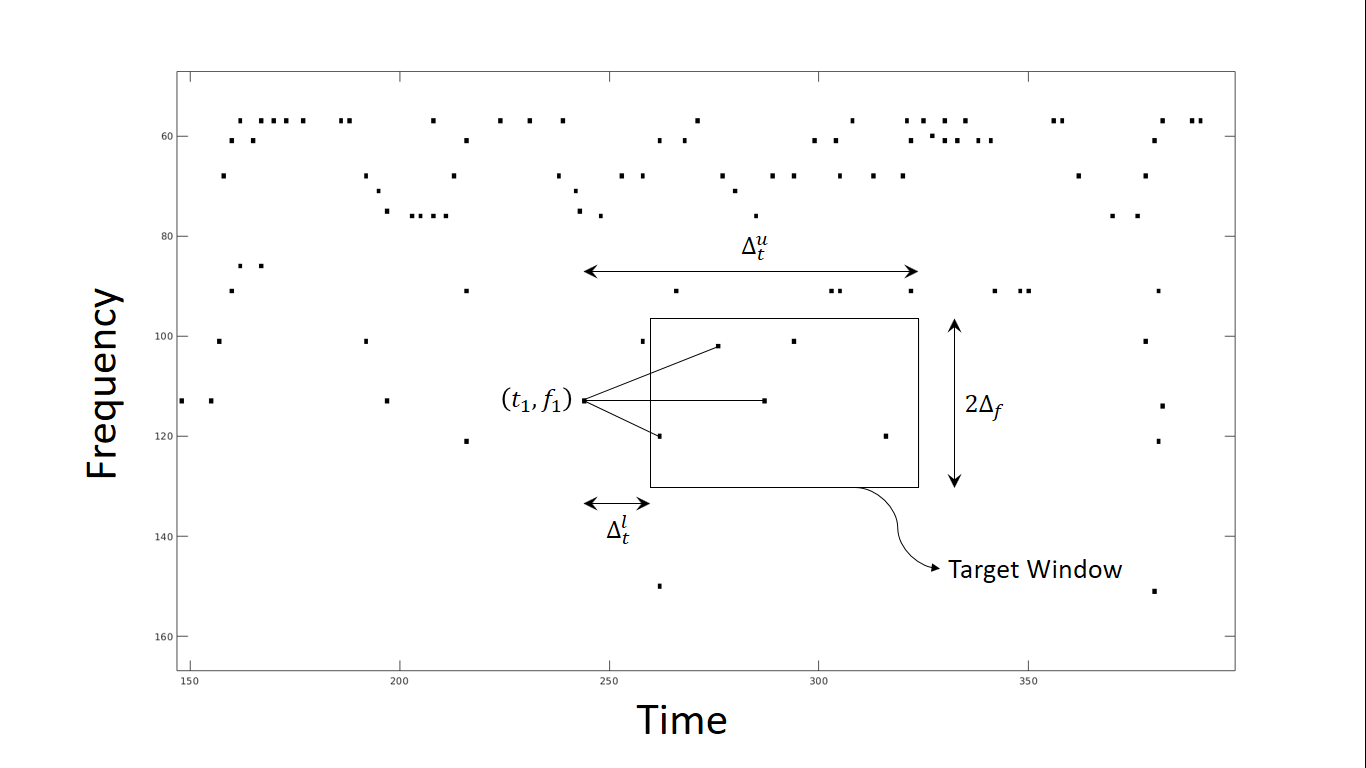
\includegraphics[width=\linewidth]{constellation-map.png}
		\caption{پیک‌های محلی اسپکتروگرام با پنجره‌ی هدف برای جفت پیک‌ها}
	\end{figure}
	
	تابع \lr{peak\_to\_pair} در اختیار شما قرار گرفته است. این تابع تنها یک ورودی می‌گیرد که ماترس \lr{peaks} است. با استفاده از تابع \lr{voiceprint} و این تابع برای فایل \lr{viva.mp3} دیاگرام تصمیم گیری را که جفت پیک‌ها با خطی به‌هم وصل شده‌اند، رسم کنید.
	 
	\section*{فاز ۲}
	در فاز بعدی این پروژه ابتدا با استفاده از توابعی که در اختیار شما قرار می‌گیرد، پایگاه داده‌ی ویژگی‌های تعدادی آهنگ را می‌سازید و سپس تابعی می‌نویسید که بهترین تطبیق برای یک کلیپ را پیدا کند. همچنین به کلیپ‌ها نویز نیز اضافه خواهید کرد و برنامه‌ی خود را با کلیپ‌های دارای نویز تست می‌کنید.
	\section*{نکات تحویل}
	فایل‌های خود را با نام \lr{P1-SID.zip} در صفحه‌ی \lr{CECM} درس بارگذاری کنید که \lr{SID} شماره‌ی دانشجویی شماست؛ برای مثال اگر شماره‌ی دانشجویی شما ۸۱۰۱۹۶۹۹۹ باشد، نام پرونده‌ی شما باید \lr{A2-810196999.zip} باشد.
	\begin{itemize}
		\item این تمرین را می‌توانید با پایتون یا متلب انجام دهید.
		\item در گزارش‌کار خود تصاویر خواسته شده در قسمت‌های \ref{ssec:spectrogram}، \ref{ssec:local-peaks}، \ref{ssec:thresholding} و \ref{ssec:construct-table} و جواب سوال‌های پرسیده شده در قسمت‌های \ref{ssec:spectrogram}، \ref{ssec:local-peaks} و \ref{ssec:thresholding} را بیاورید.
		\item اگر اسم توابعی که باید بنویسید، مشخص شده است، حتما آن را رعایت کنید.
		\item هدف این تمرین یادگیری شماست. لطفاً تمرین را خودتان انجام دهید. در صورت کشف تقلب مطابق قوانین درس با آن برخورد خواهد شد.
		\item سوالات خود را از طریق ایمیل بپرسید:
		\subitem \href{mailto:h.barkhordarpour@ut.ac.ir?subject=[SS\%20S98 P1]}{h.barkhordarpour@ut.ac.ir}
		\subitem \href{mailto:ranjbar.ali@ut.ac.ir?subject=[SS\%20S98 P1]}{ranjbar.ali@ut.ac.ir}
	\end{itemize}
\end{document}
